%%%%%%%%%%%%%%%%%%%%%%%%%%%%%%%%%%%%%%%%%
% Beamer Presentation
% LaTeX Template
% Version 1.0 (10/11/12)
%
% This template has been downloaded from:
% http://www.LaTeXTemplates.com
%
% License:
% CC BY-NC-SA 3.0 (http://creativecommons.org/licenses/by-nc-sa/3.0/)
%
% Modified by Emma K. Gagne
% 23 February 2021
%%%%%%%%%%%%%%%%%%%%%%%%%%%%%%%%%%%%%%%
\documentclass[12pt]{beamer}\usepackage[]{graphicx}\usepackage[]{color}
% maxwidth is the original width if it is less than linewidth
% otherwise use linewidth (to make sure the graphics do not exceed the margin)
\makeatletter
\def\maxwidth{ %
  \ifdim\Gin@nat@width>\linewidth
    \linewidth
  \else
    \Gin@nat@width
  \fi
}
\makeatother

\definecolor{fgcolor}{rgb}{0.345, 0.345, 0.345}
\newcommand{\hlnum}[1]{\textcolor[rgb]{0.686,0.059,0.569}{#1}}%
\newcommand{\hlstr}[1]{\textcolor[rgb]{0.192,0.494,0.8}{#1}}%
\newcommand{\hlcom}[1]{\textcolor[rgb]{0.678,0.584,0.686}{\textit{#1}}}%
\newcommand{\hlopt}[1]{\textcolor[rgb]{0,0,0}{#1}}%
\newcommand{\hlstd}[1]{\textcolor[rgb]{0.345,0.345,0.345}{#1}}%
\newcommand{\hlkwa}[1]{\textcolor[rgb]{0.161,0.373,0.58}{\textbf{#1}}}%
\newcommand{\hlkwb}[1]{\textcolor[rgb]{0.69,0.353,0.396}{#1}}%
\newcommand{\hlkwc}[1]{\textcolor[rgb]{0.333,0.667,0.333}{#1}}%
\newcommand{\hlkwd}[1]{\textcolor[rgb]{0.737,0.353,0.396}{\textbf{#1}}}%
\let\hlipl\hlkwb

\usepackage{framed}
\makeatletter
\newenvironment{kframe}{%
 \def\at@end@of@kframe{}%
 \ifinner\ifhmode%
  \def\at@end@of@kframe{\end{minipage}}%
  \begin{minipage}{\columnwidth}%
 \fi\fi%
 \def\FrameCommand##1{\hskip\@totalleftmargin \hskip-\fboxsep
 \colorbox{shadecolor}{##1}\hskip-\fboxsep
     % There is no \\@totalrightmargin, so:
     \hskip-\linewidth \hskip-\@totalleftmargin \hskip\columnwidth}%
 \MakeFramed {\advance\hsize-\width
   \@totalleftmargin\z@ \linewidth\hsize
   \@setminipage}}%
 {\par\unskip\endMakeFramed%
 \at@end@of@kframe}
\makeatother

\definecolor{shadecolor}{rgb}{.97, .97, .97}
\definecolor{messagecolor}{rgb}{0, 0, 0}
\definecolor{warningcolor}{rgb}{1, 0, 1}
\definecolor{errorcolor}{rgb}{1, 0, 0}
\newenvironment{knitrout}{}{} % an empty environment to be redefined in TeX

\usepackage{alltt}
% only 10,11, or 12 pt fonts
% PACKAGES-----------------------------------
\usepackage{graphicx} % Allows including images
\usepackage{booktabs} % Allows the use of \toprule, \midrule and \bottomrule in tables

% THEMES AND COLORS-------------------------
\mode<presentation> {
\usefonttheme{default}
% FONTTHEMES: default, structurebold, structuresmallcapsserif, structureitalicserif, serif, professionalfonts


\usetheme{Berkeley}
% THEMES: default, AnnArbor, Antibes, Bergen, Berkeley, Berlin, Boadilla, boxes, CambridgeUS, Copenhagen, Darmstadt, Dresden, Frankfurt, Goettingen, Hannover, Ilmenau, JuanLesPins, Luebeck, Madrid, Malmoe, Marburg, Montpellier, PaloAlto, Pittsburgh, Rochester, Singapore, Szeged, Warsaw

\usecolortheme{seahorse}
%COLORTHEMES: default, albatross, beaver, beetle, crane, dolphin, dove, fly, lily, orchid, rose, seagull, seahorse, sidebartab, structure, whale, wolverine 

% DISPLAY OPTIONS--------------------------
% \setbeamertemplate{footline} % To remove the footer line in all slides, uncomment this line

% \setbeamertemplate{footline}[page number] % To replace the footer line in all slides with a simple slide count, uncomment this line

% \setbeamertemplate{navigation symbols} % To remove the navigation symbols from the bottom of all slides, uncomment this line
}
% -----------------------------------------

% TITLE PAGE DATA--------------------------
\title[Bioacoustics and Stress]{Bottlenose dolphin whistles indicate less stress during COVID-19 pandemic} % The short title appears at the bottom of every slide, the full title is only on the title page

\author{Emma K. Gagne} % Your name

\institute[UVM] % Your institution as it will appear on the bottom of every slide, may be shorthand to save space
{
University of Vermont \\ % Your institution for the title page
Department of Biology \\
Burlington, VT 05401 USA \\ 
\medskip
\textit{emma.gagne@uvm.edu} % Your email address
}
\date{9 January 2021} % Date, can be changed to a custom date or \today
% -----------------------------------------

% BEGIN DOCUMENT---------------------------
\IfFileExists{upquote.sty}{\usepackage{upquote}}{}
\begin{document}

% OPTIONAL TITLE PAGE SLIDE----------------
\begin{frame}
\titlepage % Print the title page as the first slide
\end{frame}

% OPTIONAL TABLE OF CONTENTS SLIDE---------

\begin{frame}
\frametitle{Overview} % Table of contents slide, comment this block out to remove it
\tableofcontents % Throughout your presentation, if you choose to use \section{} and \subsection{} commands, these will automatically be printed on this slide as an overview of your presentation
\end{frame}

% OPTIONAL SECTION HEADERS-----------------
\section{Bottlenose Dolphin Communication} % Sections can be created in order to organize your presentation into discrete blocks; all sections and subsections are automatically printed in the table of contents as an overview of the talk

\subsection{Acoustics}
\subsection{Types of Calls} % A subsection can be created just before a set of slides with a common theme to further break down your presentation into chunks

\section{Boat Presence and Stress}

\subsection{COVID-19 Boat Presence}
\subsection{Impacts}

\section{Importance}


% SLIDE (BULLET POINTS)--------------------
\begin{frame}
\frametitle{Acoustic Communication}
\begin{itemize}
\item Dolphins produce sound using "monkey lips" in the nasal sac area.
\item This creates a sound wave.
\item This sound wave is perceived in other dolphins through conduction from the lower jaw bone to the middle ear.
\end{itemize}
\end{frame}

% SLIDE (BULLET POINTS)--------------------
\begin{frame}
\frametitle{Types of Dolphin Communication}
\begin{itemize}
\item echolocation clicks: used for finding prey
\item variant whistles: function is poorly understood
\item signature whistles: indicate individual identity similar to a name
\end{itemize}
\end{frame}

% SLIDE (SEQUENTIAL BULLET POINTS)---------
\begin{frame}
\frametitle{Importance of Signature Whistles}
\begin{itemize}
\item<1-> Identify individual identity
\item<2-> Help reconnect with conspecifics
\item<3-> Mother/calf pairs use to stay together
\end{itemize}
\end{frame}

% SLIDE (FIGURE)-----------------------------
\begin{frame}
\frametitle{Bottlenose Dolphin Audiogram Compared to Other Cetaceans}
% Uncomment the code on this slide to include your own image from the same directory as the template  file.
 \begin{figure}
   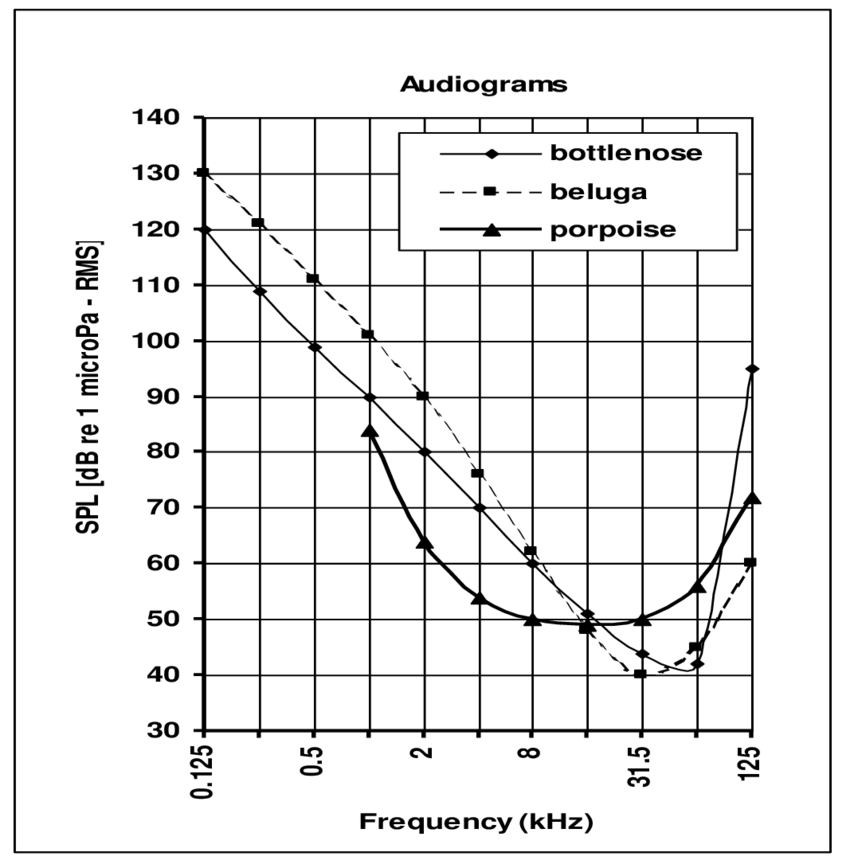
\includegraphics[width=1.0\linewidth]{Examples-of-absolute-audiograms-for-the-bottlenose-dolphin-beluga-whale-and-harbour.png}
 % use this format for absolute sizing
% 
\includegraphics[width=3cm, height=4cm]{UVMLogo.jpg}
\end{figure}
\end{frame}

% SLIDE (TABLE)----------------------------
\begin{frame}
\frametitle{Whistle Parameters}
\begin{table}
\begin{tabular}{l l l}
\toprule
\textbf{Peak Frequency} & \textbf{Delta Time} & \textbf{Inflection Points}\\
\midrule
435.23 & 2.453 & 3 \\
45.324 & 3.436 & 0 \\
564.435 & 0.352 & 1 \\
\bottomrule
\end{tabular}
\caption{Whistle Parameters from Bottlenose Dolphins}
\end{table}
\end{frame}

%------------------------------------------------
%------------------------------------------------
% SLIDE (PARAGRAPHS OF TEXT)---------------
\begin{frame}
\frametitle{Noise Masking}
Noise masking occurs when other objects in the acoustic field overlap with the same frequency an organism is communicating at.\\~\\

Organisms may avoid noise masking by changing the frequency of their calls, the number of time they call, or the duration of their calls to better be heard. This fits with the acoustic adaptation hypothesis. 
\end{frame}

% SLIDE (BLOCKS OF HIGHLIGHTED TEXT)-------
\begin{frame}
\frametitle{Acoustic Adaptation Hypothesis}
\begin{block}{Theory}
Individuals are more successful when their signals can be received. This requires being able to avoid masking.
\end{block}

\begin{block}{Example}
Frogs lower their call frequency in the presence of busy and loud highways.
\end{block}

\begin{block}{Importance}
This determines individual fitness.
\end{block}
\end{frame}

% SLIDE (EMBEDDED R CODE)------------------
\begin{frame}[fragile]{Embedded R Code; \texttt{fragile} frame}
\begin{block}

\begin{knitrout}
\definecolor{shadecolor}{rgb}{0.969, 0.969, 0.969}\color{fgcolor}\begin{kframe}
\begin{alltt}
\hlcom{# show some output...}
\hlkwd{runif}\hlstd{(}\hlnum{10}\hlstd{)}
\end{alltt}
\begin{verbatim}
##  [1] 0.08727965 0.61932732 0.36822169 0.54319136 0.55205928 0.76759529
##  [7] 0.67598206 0.69736277 0.46447823 0.53577535
\end{verbatim}
\end{kframe}
\end{knitrout}

\end{block}
\end{frame}

% SLIDE (EMBEDDED R FIGURE)----------------
\begin{frame}[fragile]{Embedded R Figure; \texttt{fragile} frame}
\begin{block}

\begin{knitrout}
\definecolor{shadecolor}{rgb}{0.969, 0.969, 0.969}\color{fgcolor}

{\centering 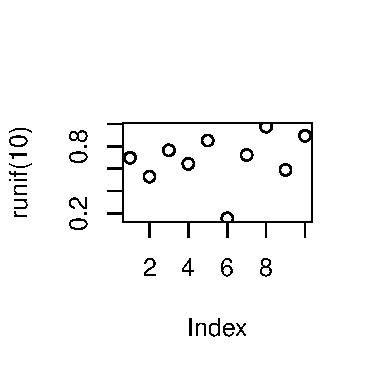
\includegraphics[width=\maxwidth]{figure/unnamed-chunk-2-1} 

}



\end{knitrout}

\end{block}
\end{frame}

% SLIDE (FINAL SLIDE)------------------------
\begin{frame}
\Huge{\centerline{The End}}
\end{frame}

%------------------------------------------------
\end{document}
